\documentclass [titlepage,12pt,letter] {article}
\pagestyle{myheadings}


\usepackage{graphicx} 
\usepackage{epsfig}
\usepackage{subfigure}
\usepackage{fancyhdr}
\usepackage{url} 
\usepackage{amsmath}
\usepackage{algorithm} 
\usepackage{algorithmic}
\usepackage{gensymb}
\usepackage{breqn}
\pagestyle{fancy}



\fancyhead{}
\fancyfoot{}
			
\lhead{CSC349A Lecture Notes}
\rhead{Little, Rich}


\setcounter{page}{1}
\cfoot{\thepage}




\begin{document} 


These are the lecture notes for CSC349A Numerical Analysis taught by
Rich Little. They roughly correspond to
the material covered in each lecture in the classroom but the actual
classroom presentation might deviate significantly from them depending
on the flow of the course delivery. They are provide as a reference to
the instructor as well as supporting material for students who miss
the lectures. They are simply notes to support the lecture so the text
is not detailed and they are not thoroughly checked. Use at your own
risk. They are complimentary to the handouts. Many thanks to all the
guidance and materials I received from Dale Olesky who has taught this
course for many years and George Tzanetakis.


\section{Approximation Theory/Curve Fitting} 

Our next topic is the study of how a given function can be approximated by another function 
from a sspecified class of functions. The given function may be discrete or continuous. 

Typically the approximating function exhibits some desired properties such as: 

\begin{enumerate} 
\item{Continuity} 
\item{Easily differentiated} 
\item{Easily integrated} 
\item{Easily evaluated} 
\end{enumerate}

Common classes of approximating functions: 
\begin{enumerate} 
\item{Polynomials} 
\item{Piecewise polynomials (splines)}
\item{Trigonometric sums (fourier series)}
\end{enumerate} 

We will also study criteria for what constitutes a ``good'' approximating function. 

\section{Polynomial interpolation} 

Recall that the general formula for an $n$th-order polynomial is
\[
f(x) = a_0 + a_1x + \dotsm + a_nx^n
\]
\noindent 
For $n+1$ distinct data points there is one and only one order $n$ (or less) polynomial that passes through them all. That is,
\begin{itemize}
\item{only one line that passes through two points}
\item{only one parabola that passes through three points, etc}
\end{itemize}
{\bf Polynomial Interpolation} consists of determining the unique $n$th-order polynomial that fits the $n+1$ data points in question.
\begin{itemize}
\item{Although the polynomial is unique there are different methods for finding it and different formats for expressing it.}
\end{itemize}

\noindent
{\bf Formally:}

Let $y=f(x)$ be any given function. For any value of $n \geq 0$ and any given values 
$x_0, x_1, \dots, x_n$, let $y_i = f(x_i)$. The {\bf polynomial interpolation problem} 
is to determine a polynomial $P(x)$ of degree less or equal to $n$ for which: 
\[
P(x_i) = y_i \;\;\; \mbox{for } i=0,1,\dots,n 
\]
\noindent 
The set of $n+1$ data point $(x_i,y_i)$ maybe the only functional values known (that is, $f(x)$ is 
a {\bf discrete function}, which could occur for example with experimental data), or $f(x)$ maybe be a known {\bf continuous function}, and the $n+1$ data points $(x_i, y_i)$ are a finite set of values with $y_i = f(x_i)$. 

If $z$ is some value between 2 of the given value $x_i$ and if $P(z)$ is computed as an approximation to $f(z)$, then this approximation to $f(z)$ is said to be determined by polynomial {\bf interpolation}. 

On the other hand, if $z$ lies outside of the interval containing all of the value $x_i$ and if $P(z)$ is computed as an approximation to $f(z)$, then this approximation to f(z) is said to be determined by polynomial {\bf extrapolation}. 

Note that an {\bf interpolating polynomial} and the {\bf Taylor polynomial} both determine polynomial approximations to $f(x)$. However, in general they are very different approximations to $f(x)$. Note that an interpolating polynomial uses the information: 

\[
y_0 = f(x_0), y_1 = f(x_1), \dots, y_n = f(x_n)
\]
\noindent 
to determine the polynomial approximation, whereas the Taylor polynomial uses the information: 
\[
f(x_0), f'(x_0), \dots, f^{(n)}(x_0)
\]
\noindent 
to determine the polynomial approximation. 

\section{Lagrange Interpolating Polynomial} 

Given ${(x_i,f(x_i))}, 0 \leq i \leq n$, with all $x_i$ distinct, consider the function: 
\begin{align*}
P(x) &= \sum_{i=0}^{n} L_i(x) f(x_i) \\
     &= L_0(x) f(x_0) + L_1(x)f(x_1) + \dots + L_n(x)f(x_n)
\end{align*} 
\noindent 
where 
\begin{align*}
L_i(x) &= \frac{(x-x_0)(x-x_1)\dots(x-x_{i-1})(x-x_{i+1})\dots(x-x_n)}{(x_i-x_0)(x_i-x_1)\dots(x_i-x_{i-1})(x_i-x_{i+1})\dots(x_i-x_n)} \\
   &= \prod_{j=0,j \neq i}^{n} \frac{x-x_j}{x_i-x_j}, \;\;\; \mbox{for } i=0,1,2,\dots,n 
\end{align*}

\subsection{Example 1}

Derive the general, order $n=1$, Lagrange interpolating polynomial.

\begin{align*}
P(x) &= \sum_{i=0}^{1} L_i(x) f(x_i) \\
     &= L_0(x) f(x_0) + L_1(x)f(x_1) \\
     &= \prod_{j=0,j \neq 0}^{1} \frac{x-x_j}{x_0-x_j} f(x_0) + \prod_{j=0,j \neq 1}^{1} \frac{x-x_j}{x_1-x_j} f(x_1) \\
     &= \frac{x-x_1}{x_0-x_1} f(x_0) + \frac{x-x_0}{x_1-x_0} f(x_1)
\end{align*}

\subsection{Example 2}
Derive the general, order $n=2$, Lagrange interpolating polynomial.

\begin{align*}
P(x) &= \sum_{i=0}^{2} L_i(x) f(x_i) \\
     &= L_0(x) f(x_0) + L_1(x)f(x_1) + L_2(x)f(x_2)
\end{align*}

\noindent
where each $L_i(x)$ is at most a second degree polynomial given by,

\begin{align*}
   L_0(x) &= \prod_{j=0,j \neq 0}^{2} \frac{x-x_j}{x_0-x_j} = \frac{(x-x_1)(x-x_2)}{(x_0-x_1)(x_0-x_2)} \\
   L_1(x) &= \prod_{j=0,j \neq 1}^{2} \frac{x-x_j}{x_1-x_j} = \frac{(x-x_0)(x-x_2)}{(x_1-x_0)(x_1-x_2)} \\ 
   L_2(x) &= \prod_{j=0,j \neq 2}^{2} \frac{x-x_j}{x_2-x_j} = \frac{(x-x_0)(x-x_1)}{(x_2-x_0)(x_2-x_1)} \\
\end{align*}

\noindent
Therefore,
\begin{dmath}
P(x) = \frac{(x-x_1)(x-x_2)}{(x_0-x_1)(x_0-x_2)}f(x_0) + \frac{(x-x_0)(x-x_2)}{(x_1-x_0)(x_1-x_2)}f(x_1) + \frac{(x-x_0)(x-x_1)}{(x_2-x_0)(x_2-x_1)}f(x_2)
\end{dmath}

Note here that $L_0(x_0) = 1$ and both $L_0(x_1) = L_0(x_2) = 0$. Similarly for $L_1$ and $L_2$.

Since each function $L_i(x)$ is a polynomial of order $n$ and $f(x_i)$ is a constant, $P(x)$ is a polynomial of order $\leq n$. Since 
\[
L_i(x_i) = 1 \mbox{ and } L_i(x_j) = 0 \mbox{ if } j \neq i,
\]
\noindent 
it follows that: 
\[
P(x_i) = f(x_i), \;\;\; \mbox{ for } i=0,1,2,\dots, n
\]
\noindent 
that is, $P(x)$ is a an interpolating polynomial for the given data. It is called the {\bf Lagrange interpolating polynomial}. 

\subsection{Example 3}
Evaluate $\ln(2)$ using Lagrange polynomial interpolation, given that
\begin{align*}
\ln{1} &= 0 \\
\ln 4 &= 1.386294 \\
\ln 6 &= 1.791760
\end{align*}

Here, $x_0 = 1, x_1=4, x_2=6$ and $f(x_0)=0, f(x_1)=1.386294, f(x_2)=1.791760$. Substituting these into equation (1) above gives,

\begin{dmath*}
P(x) = \frac{(x-x_1)(x-x_2)}{(x_0-x_1)(x_0-x_2)}f(x_0) + \frac{(x-x_0)(x-x_2)}{(x_1-x_0)(x_1-x_2)}f(x_1) + \frac{(x-x_0)(x-x_1)}{(x_2-x_0)(x_2-x_1)}f(x_2) \\
  = \frac{(x-4)(x-6)}{(1-4)(1-6)}0 + \frac{(x-1)(x-6)}{(4-1)(4-6)}(1.386294) + \frac{(x-1)(x-4)}{(6-1)(6-4)}(1.791760) 
\end{dmath*}

and thus,

\begin{dmath*}
P(2) = \frac{(2-4)(2-6)}{(1-4)(1-6)}0 + \frac{(2-1)(2-6)}{(4-1)(4-6)}(1.386294) + \frac{(2-1)(2-4)}{(6-1)(6-4)}(1.791760) 
  = \frac{-4}{3(-2)}(1.386294) - \frac{2}{5(2)}(1.791760)
  = 0.565844
\end{dmath*}

I ran the following script in MATLAB to illustrate the above example. The plot produced by this is given in Figure 1.

\begin{verbatim}
x = [0 : 0.01 : 8];
y = log(x);
L0x = 0;
L1x = -0.231049.*(x.^2-7.*x+6);
L2x = 0.179176 .* (x.^2-5.*x+4);
Px = L1x+L2x;
plot(x,y)
plot(x,y,x,Px)
plot(x,y,x,Px,x,L0x,x,L1x,x,L2x)
plot(x,y,'r',x,Px,'b',x,L0x,'y',x,L1x,'g',x,L2x,'c')
\end{verbatim}

\begin{figure} 
  \centering
  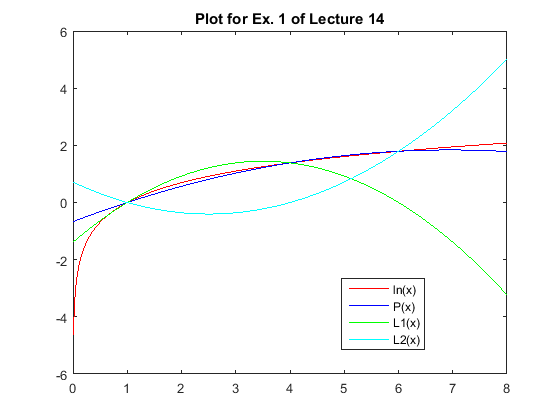
\includegraphics[scale=0.75]{lagrange_example}
  \caption{Plot of the Lagrange polynomial for $\ln(x)$ plus the individual $L_i(x)$ polynomials used in its construction}
  \label{fig:lagrange}
\end{figure}

\subsection{Example 4} 
A complete elliptic integral function of the first kind is defined by
\[
K(k) = \int_{0}^{\pi/2} \frac{dz}{\sqrt{1 - k^2\sin^2{z}}}
\]
Interpolate $K(\sin{65.5 \degree})$ where
\begin{center}
\begin{tabular}{c|c} 
$\sin^{-1}{k}$ & $K(k)$ \\
 \hline
 $65\degree$ & $2.3088$ \\ 
 $66\degree$ & $2.3439$ \\ 
 $67\degree$ & $2.3809$ \\ 
\end{tabular}
\end{center}

Here, we use $x_0 = 65, x_1=66, x_2=67$ and $f(x_0)=2.3088, f(x_1)=2.3439, f(x_2)=2.3809$. Substituting these into equation (1) above gives,

\begin{dmath*}
P(x) = \frac{(x-x_1)(x-x_2)}{(x_0-x_1)(x_0-x_2)}f(x_0) + \frac{(x-x_0)(x-x_2)}{(x_1-x_0)(x_1-x_2)}f(x_1) + \frac{(x-x_0)(x-x_1)}{(x_2-x_0)(x_2-x_1)}f(x_2) \\
  = \frac{(x-66)(x-67)}{(65-66)(65-67)}(2.3088) + \frac{(x-65)(x-67)}{(66-65)(66-67)}(2.3439) + \frac{(x-65)(x-66)}{(67-65)(67-66)}(2.3809) 
\end{dmath*}

and thus,

\begin{dmath*}
P(65.5) = \frac{(65.5-66)(65.5-67)}{(65-66)(65-67)}(2.3088) + \frac{(65.5-65)(65.5-67)}{(66-65)(66-67)}(2.3439) + \frac{(65.5-65)(65.5-66)}{(67-65)(67-66)}(2.3809) 
  = \frac{(-0.5)(-1.5)}{2}(2.3088) + \frac{(0.5)(-1.5)}{-1}(2.3439) + \frac{(0.5)(-0.5)}{2}(2.3809) 
  = 0.8658+1.757925-0.2976125
  = 2.3261125
\end{dmath*}

Therefore, when $\sin^{-1}(k)=65.5 \degree$, then $K(k)=2.3261125$. Fun fact, when you do this in MATLAB to confirm you get the following,

\begin{verbatim}
>> k = sind(65.5)

k =

   0.909961270876543

>> syms z
>> int(1/sqrt(1 - k^2 * (sin(z))^2), z, 0,(pi/2))
 
ans =
 
ellipticK(3729113412932597/4503599627370496)

>> ellipticK(3729113412932597/4503599627370496)

ans =

   2.326123965501425
\end{verbatim}

\end{document} 















